\documentclass{article}
\usepackage[utf8]{inputenc}
\usepackage{hyperref}

\usepackage{graphicx}
\usepackage{subcaption}

\graphicspath{ {./images/} }
\usepackage{wrapfig}
\usepackage{float}

\usepackage{caption}
\captionsetup[figure]{font=footnotesize}

\usepackage[framemethod=TikZ, xcolor=RGB]{mdframed}
\definecolor{mycolor}{RGB}{225,225,225}
\newmdenv[
        linecolor=mycolor,
        topline=false,
        bottomline=false,
        rightline=false,
        linewidth=1pt,
        innerleftmargin=5pt,
        leftmargin=0pt,
        rightmargin=0pt,
        innerbottommargin=0pt
]{separator}

\usepackage[backend=biber,
bibencoding=ascii,
style=ieee,
citestyle=numeric,
sorting=ynt
]{biblatex}
\addbibresource{bibliography.bib}

\title{Collaborative Learning: \\
    \normalsize Strategies and Platform Development
}
\author{Paul A. Baier \\ 
    \footnotesize CSIS 698 - Project Thesis \\
    \footnotesize Dr. Ayman Hajja
}
\date{April 20, 2020}

\begin{document}

\maketitle

\section{Introduction and Motivation}
    A Student Response System (SRS) is a tool used in classrooms to get student feedback in real time. Typically it would be an online tool that teachers can set up with questions and present to students, and students can connect and answer the questions providing real time results. Gamification is the process of applying learning outcomes to games. The goal of this project is to create a fully customizable and programmable gamified SRS platform. We categorize such a system as a ``Student Response Game'' (SRG).
    \smallskip

    We decided to create a flexible, programmable SGR because, while similar games exist, we found them limiting in the game options they offers. The idea originated with student collaboration in mind because the existing platforms' team modes leave a lot to be desired. As we iterated over different designs and features to include we eventually arrived at the idea that users (teachers) should be able to program the game and its features to do whatever they want it to do. With this concept at the core of our platform, we designed an open system with all of the game logic and data exposed to the user. There are default behaviors built into the system for those that want a hassle free experience, but for the more ambitious and/or particular, the default behavior can be overridden and programmed in any number of different ways.  

\section{Literature Review}
    In order to identify prior work in the area of educational games we looked at roughly 2000 proceedings from the Frontiers in Education (FIE) conference from 2015-2019 and other conferences. Our search terms started with the names of similar platforms we were aware of and then within those search results we identified other similar platforms. We then recursively searched for those other platforms and built an extensive list of related work. This search method allowed us to determine other popular platforms researchers were testing that are comparable to our platform as well as other SRS/SRG platforms in development. Our search revealed some of the most popular and relevant SRGs currently in production are Kahoot \cite{kahoot}, Socrative \cite{socrative}, Quizizz \cite{quizizz}, and Quizlet \cite{quizlet}. There were also two platforms in development by researchers called Quipid \cite{quipid} and Dysgu \cite{dysgu}.

    \subsection{Kahoot} \label{kahoot}
        Kahoot is a platform that allows teachers to write questions and organize them together to create a game called a ``kahoot''. When played, the teacher projects the questions to the students, as seen in Figure \ref{fig:kahoot-question} and the students answer the questions on their own devices. The quicker a student answers the question, the more points they get. No points are awarded or subtracted for incorrect answers. After each question the results are displayed for that question and then the scoreboard with each player's cumulative score is displayed, as in Figures \ref{fig:kahoot-post_question} and \ref{fig:kahoot-scoreboard} respectively. When the game is finished an animation plays and the final results are displayed as shown in Figure \ref{fig:kahoot-final}.
        
        \begin{figure}[ht]
            \centering
            \begin{subfigure}[b]{0.49\textwidth}
                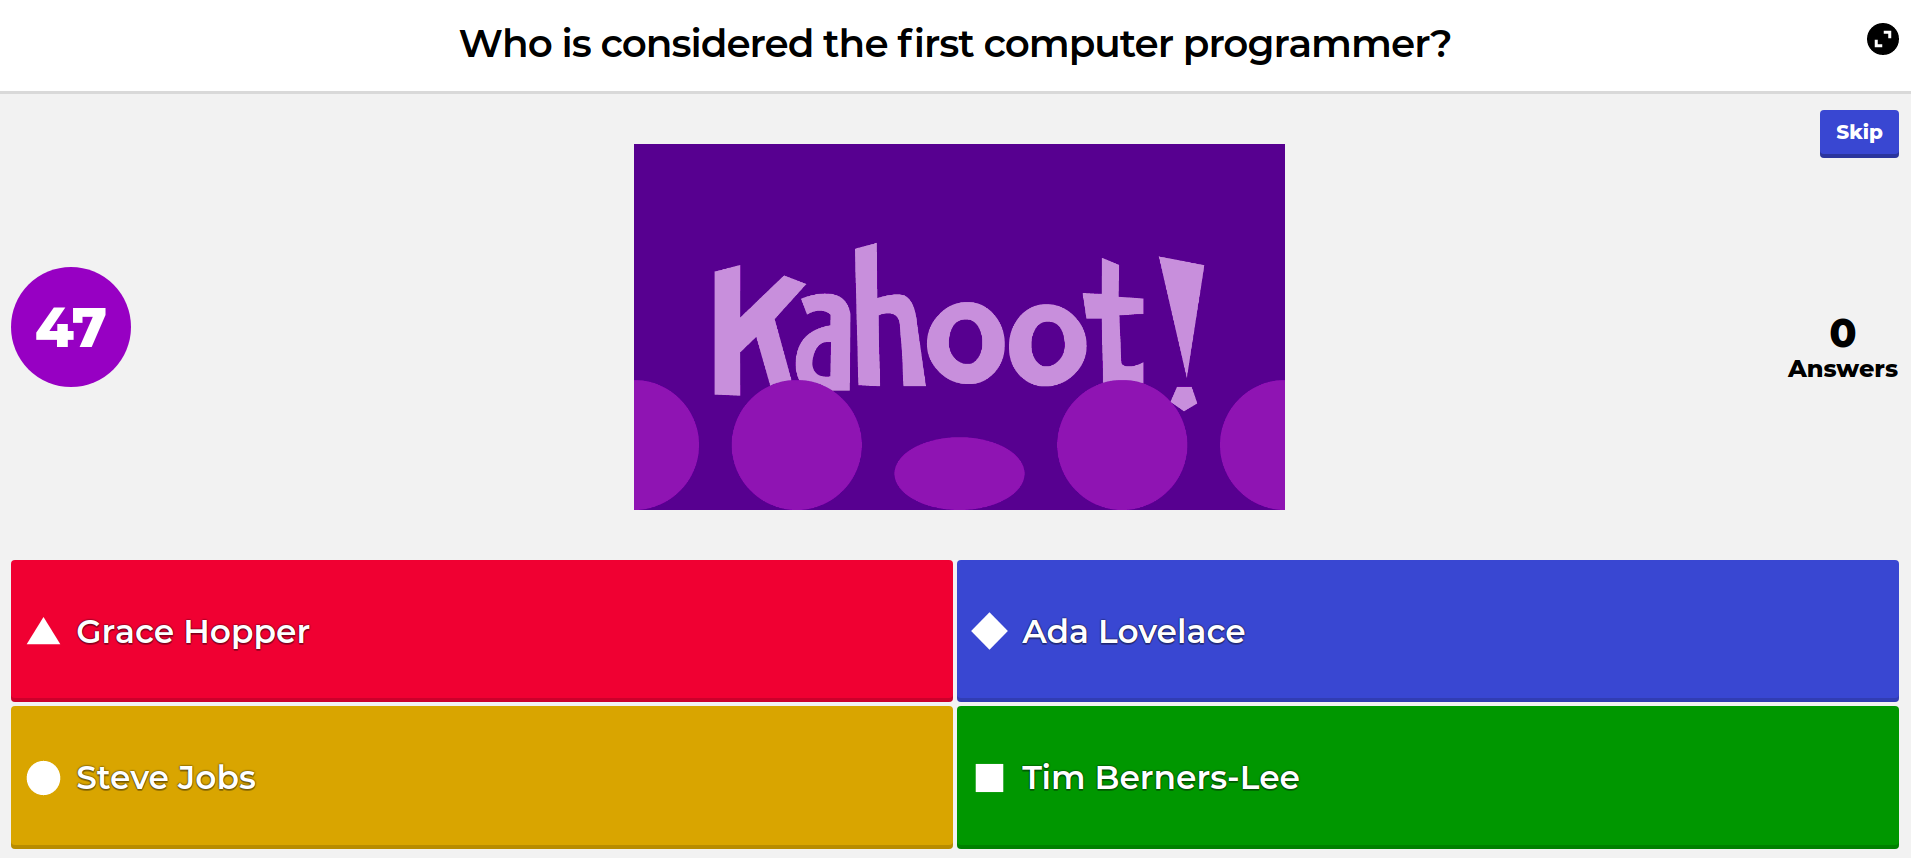
\includegraphics[width=\textwidth]{images/kahoot-question.png}
                \caption{Multiple Choice Question}
                \label{fig:kahoot-question}
            \end{subfigure}
            \begin{subfigure}[b]{0.49\textwidth}
                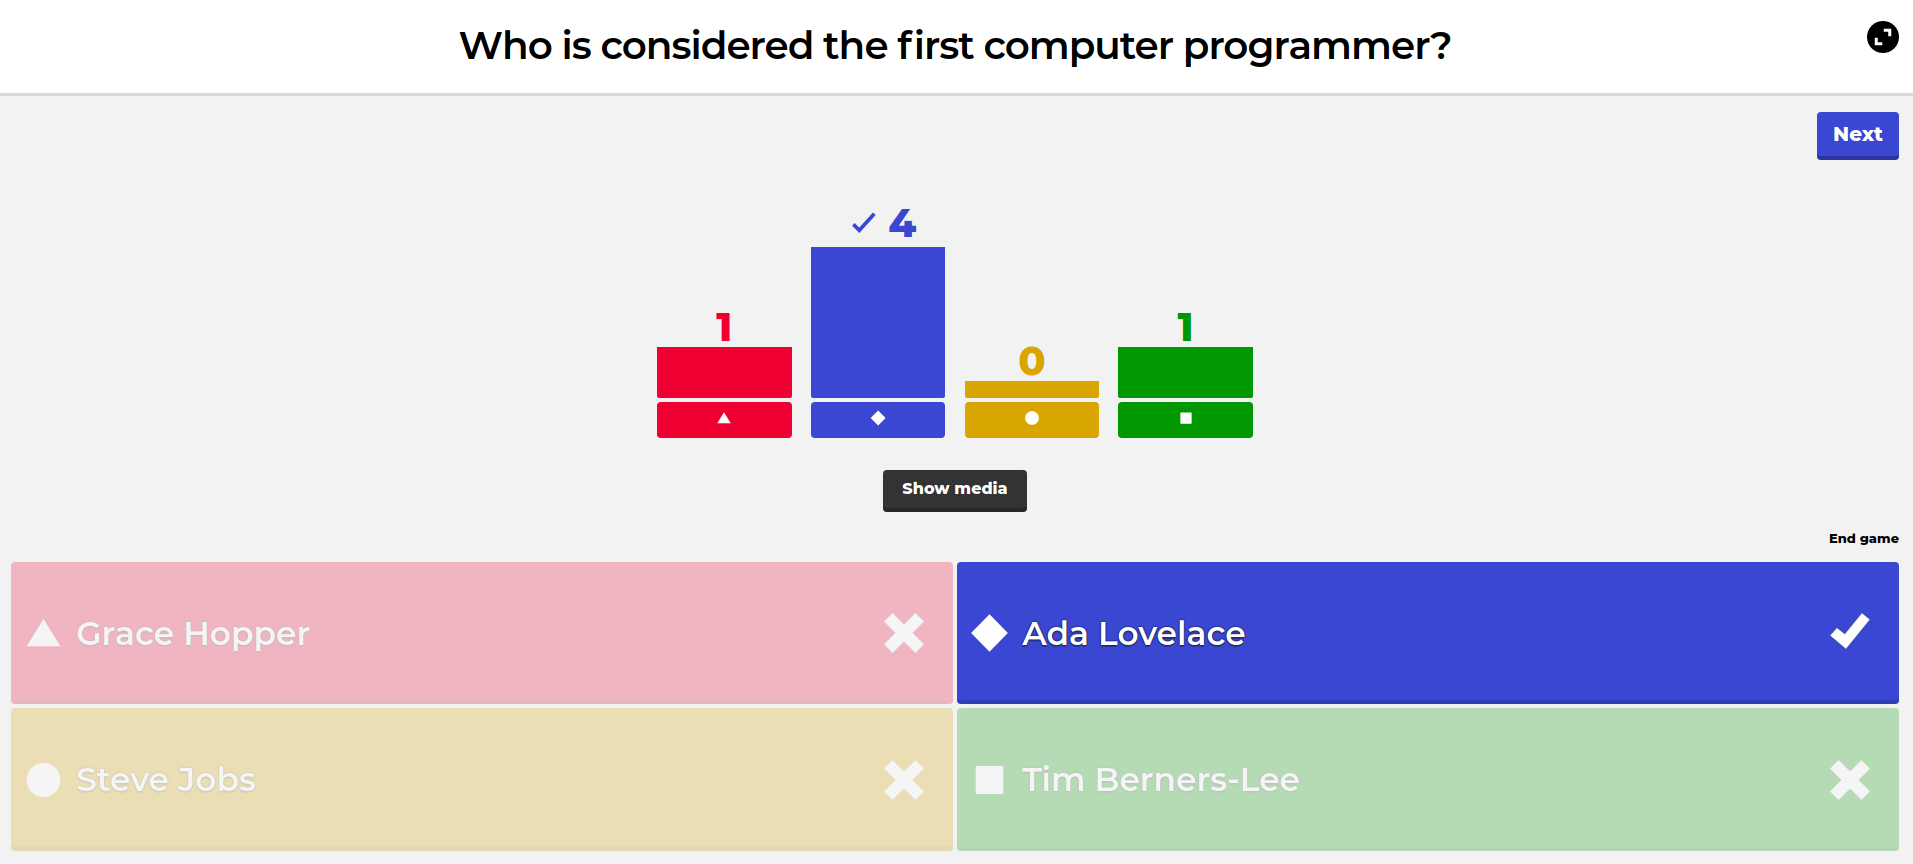
\includegraphics[width=\textwidth]{images/kahoot-post_question.png}
                \caption{Question Results}
                \label{fig:kahoot-post_question}
            \end{subfigure}
            \\
            \begin{subfigure}[b]{0.49\textwidth}
                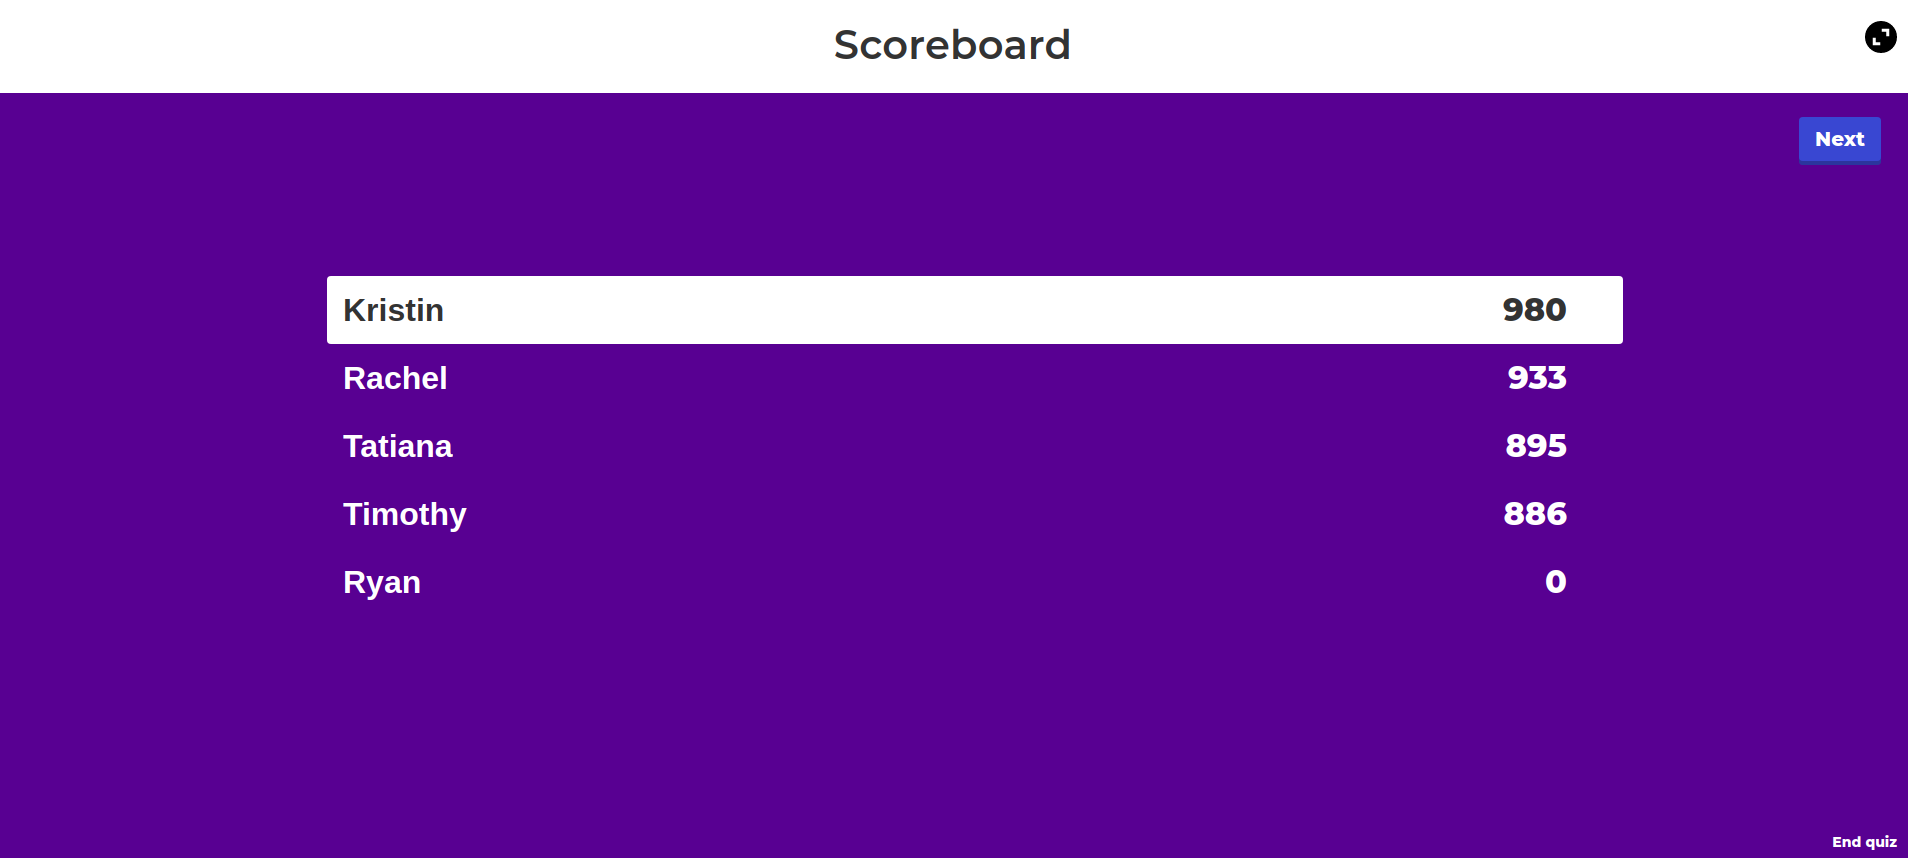
\includegraphics[width=\textwidth]{images/kahoot-scoreboard.png}
                \caption{Scoreboard}
                \label{fig:kahoot-scoreboard}
            \end{subfigure}
            \begin{subfigure}[b]{0.49\textwidth}
                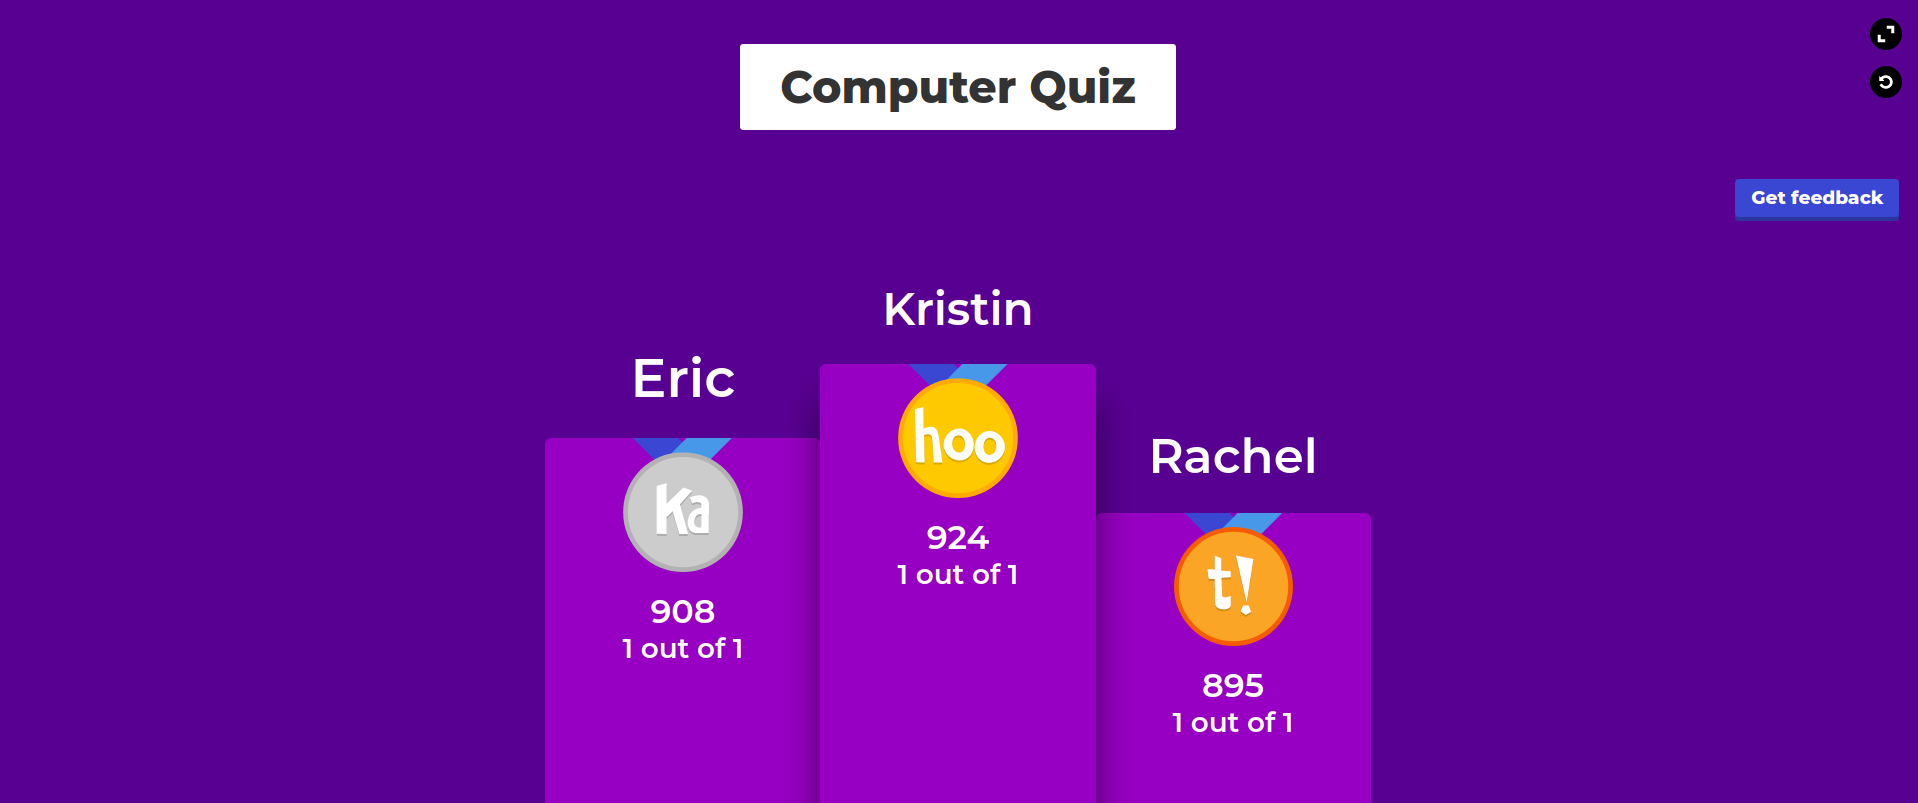
\includegraphics[width=\textwidth]{images/kahoot-finished.png}
                \caption{Final Results}
                \label{fig:kahoot-final}
            \end{subfigure}
            \caption{Kahoot Screens \cite{kahoot}}\label{fig:kahoot}
        \end{figure}
        
        When creating questions teachers are given six choices for the type of question they want to create: multiple choice, true/false, open-ended (players write in their answer), puzzle (players need to order the answers correctly), poll (no points awarded, simply polling the players), and slide, which is not a question but rather a screen with text to display more information. Each question has text and teachers are given the option to include a picture or YouTube video.
        \smallskip
        
        A Kahoot can be played live in the classroom or assigned to students to complete at their own pace. If assigned, the teacher needs to enter a due date and can set a few game options including randomize the questions, randomize the answers in each question, and use the question timer. Live games can be played in either classic mode, where students compete individually, or team mode. The difference between the two modes is that students share a device in team mode. Game options include randomizing the question and answers (like in the assigned option) and automatically moving through the questions instead of the teacher needing to click the ``next'' button as seen in Figure \ref{fig:kahoot-scoreboard}.

    \subsection{Quizizz}
        Of the existing platforms, Quizizz most resembles Kahoot and has many customizable features. The main difference between it and Kahoot or our platform is that students move through the quiz at their own pace, limited by the time assigned to each question.
        \smallskip
        
        To get started, a teacher can either choose a preexisting quiz from a library of quizzes organized by topic or they can create their own. If they choose a pre-made quiz, they can use it as is or copy and edit it to their liking. If they choose to create a new quiz, they can search through existing quizzes for questions in addition to creating their own.
        \smallskip
        
        Question types include multiple choice, checkbox (select all the correct answers), fill-in-the-blank, polls, and open-ended (the last two are ungraded but marked as correct in reports). For each question the teacher can specify the amount of time the student has to answer. Scores for answering a question correctly are determined in part by the time it took the student to answer relative to the time length of the question. However, the timer can be disabled in which case the time factor would not be considered when scoring a question.
        \smallskip
        
        Once the quiz is made there are three game modes: team, classic, and test. We will only look at team and classic modes as test mode is beyond the scope of our work.
        \smallskip
        
        Team mode, as the name suggests, organizes students into teams. In classic mode each student competes by themselves. The main difference between the two modes is that the number of teams needs to be specified by the teacher in team mode and the team scores are based on the cumulative results of the team members. Both team and classic mode share similar gameplay settings. A teacher is able to toggle the timer on or off for the game, shuffle the questions, shuffle the answer options, and allow for a ``redemption question'' where students are able to retry missed questions. There are also memes that show up between questions that the teacher can toggle off for the game or the student can toggle off for their own experience. Another option teachers have is to either show the correct answer to the student in the game after they answer, show only if the got the question right or wrong, or do not visually indicate a correct or incorrect answer (there is a noise that indicates correct or incorrect regardless of this setting).
        \smallskip
        
        Lastly Quizizz has a feature called ``Power-ups'' which ``are single-use abilities designed to increase engagement and participation'' \cite{quizizz}. Currently there are nine power-ups that are awarded sporadically to players. Once awarded, an icon appears on the student's screen and they can use it any time by clicking on the icon. An example of a power up is 50-50 which eliminates half of the incorrect answers. This entire system is available in both team and classic mode and can be disable before starting the game.
        \smallskip
        
        Described above are only some of the features offered on the Quizizz platform but they represent the most relevant when compared with our design.
    
    \subsection{Socrative}
        Socrative is a web application focused on student engagement and tracking. It offers a number of features outside of the scope of our application, however one of its activities, called ``Space Race'', is comparable.
        \smallskip
        
        Space Race is a quiz-like game where students are asked a series of questions prearranged by the teacher. Figure \ref{fig:socrative-space-race} shows how student progress is tracked by little rocket ships (or other icons) that move across the teacher's dashboard when a question is answered correctly. The goal is to be the first individual or team to have their rocket reach across the screen.
        \smallskip
        
        \begin{figure}[ht]
            \centering
            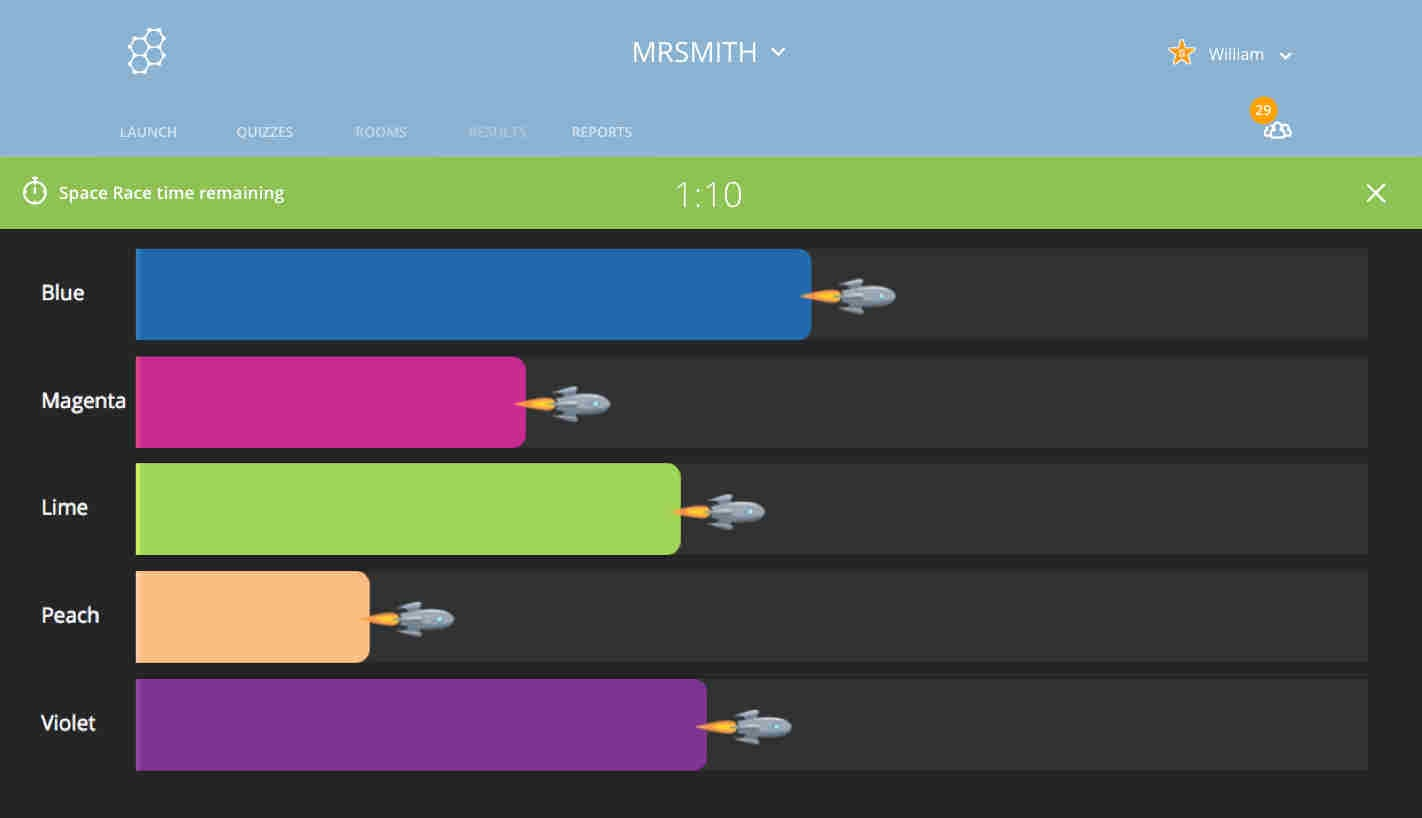
\includegraphics[width=0.8\textwidth]{images/socrative-space_race.jpg}
            \caption{Socrative Space Race \cite{socrative}}
            \label{fig:socrative-space-race}
        \end{figure}
        
        Quizzes can be made of multiple choice, true/false, and short answer questions. Other quiz options include the number of teams, how the players are assigned to teams (auto-assigned or student's choice), if the quiz is timed, shuffle the questions, shuffle the answers, show question feedback, show the final score, and if questions can only be attempted once.
    
    \subsection{Quizlet}
        Like Socrative, Quizlet is a web application that offers many features to its users. It provides students and teachers with the tools to create interactive study materials based on ``sets'', which are essentially digital flashcards. Each set is made up of any number of ``cards'' which contain a term ``side'' and a definition ``side''. Teachers and students can input the term and definition for their cards and create their own sets.
        \smallskip
        
        While most of the features offered by Quizlet do not overlap with our platform there is one, called ``Quizlet Live'', that is similar.
        \smallskip
        
        Quizlet live is a game that asks students multiple choice questions. Figure \ref{fig:quizlet-live} is the view from the teacher's dashboard that tracks student progress in real time. The teacher selects the set they want to use for the game and is able to choose between individual and team mode. Once selected, the teacher is given the option for the questions to be generated based on the term side of the card or the definition side. The game ends for everyone when the first individual or team answers all of the questions correctly. If a question is answered incorrectly the correct answer is shown and the individual or team starts back at the beginning. Questions are randomly displayed to each player/team. In individual mode there are always four answer options shown in a random order, three of which are answers for other questions in the set.
        
        \begin{figure}[ht]
            \centering
            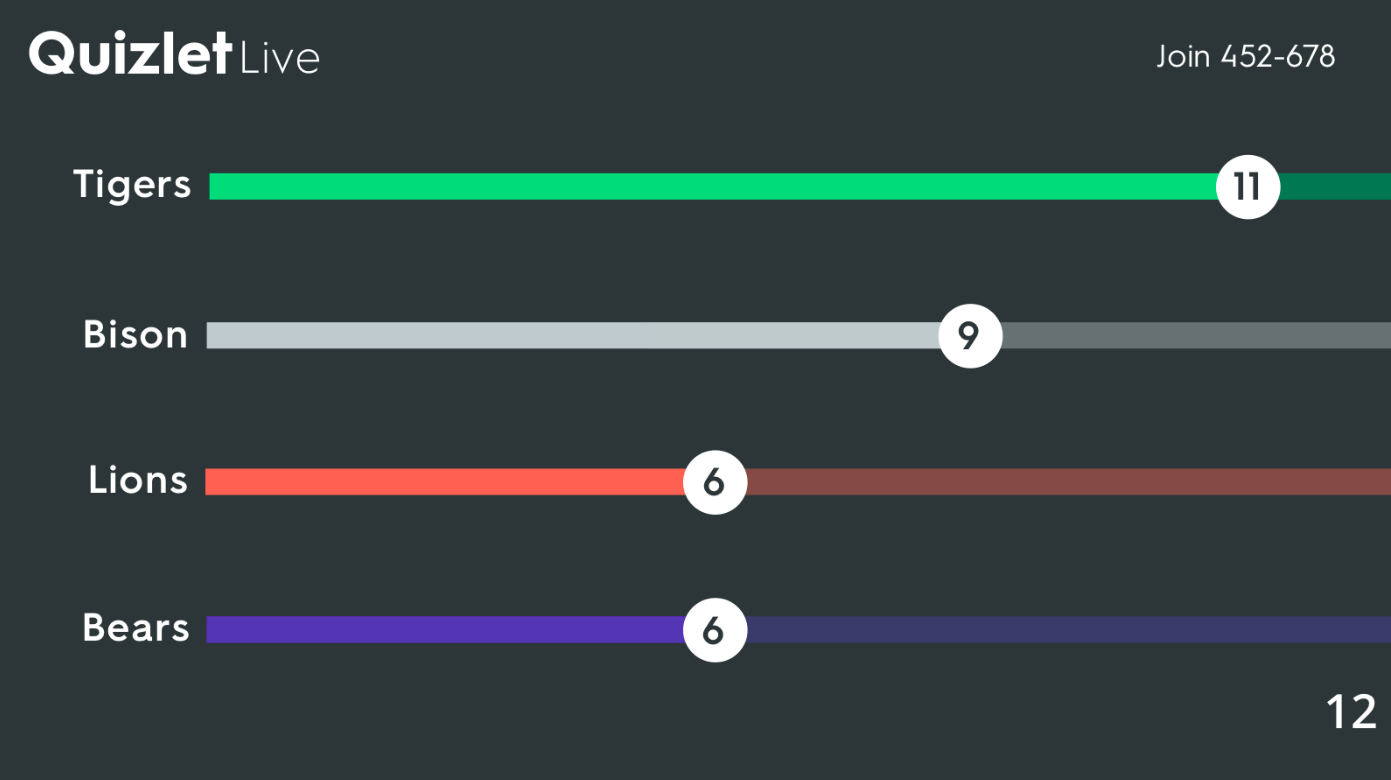
\includegraphics[width=0.5\textwidth]{images/quizlet-live.png}
            \caption{Quizlet Live Dashboard \cite{quizlet}}
            \label{fig:quizlet-live}
        \end{figure}
        
        In team mode the number of teams is automatically generated based on the number of players. Students are assigned to a team randomly and the teams
        \begin{wrapfigure}{l}{0.20\textwidth}
            \centering
            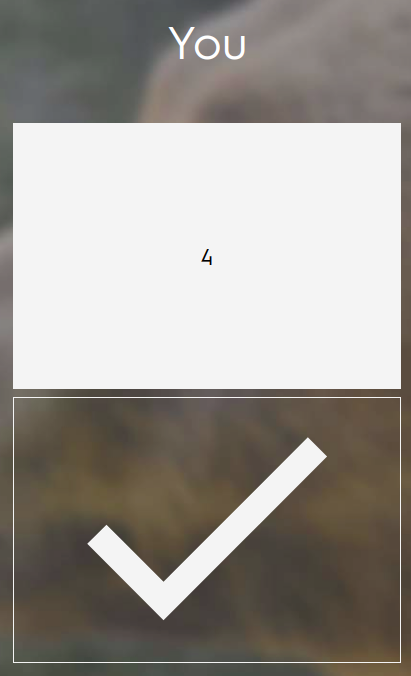
\includegraphics[width=0.10\textwidth]{images/quizlet-team.png}
            \caption{Quizlet Team View \cite{quizlet}}
            \label{fig:quizlet-team}
        \end{wrapfigure}
        can be shuffled by the teacher before the game starts. In the game, the answers to each question are split equally between each member of the team and always displayed on the screen. There are no wrong answers displayed in team mode.
        Figure \ref{fig:quizlet-team} shows an example of one player's screen with two answer options, one of which has already been submitted correctly and replaced with a check mark. The other answer option, ``4'', will need to be used in an upcoming question.
        \smallskip
        
        To illustrate the point further, if there were 10 questions and two people on one team, then each person on that team would see five answers on their screen. Each answer is the answer to one of the questions but because the answers are divided across all team members, a player will not always have the answer to a question on their screen. It is up to the player with the correct answer to answer the question. Once the question is answered correctly a check mark appears where that answer used to be and the next question is displayed.
    
    \subsection{Quipid}
        A tool that was presented at the FIE 2017 conference is called Quipid. Its purpose is to provide students with rapid feedback on assessments and teachers with a simple way to create and assign assessments. It is not a game, so it does not directly relate to our platform, however it allows teachers to create custom questions and has a programmable element which makes it related and unique relative to other platforms we looked at.
        \smallskip
        
        Quipid uses Google Sheets and Google Forms as a front end for the platform. The teacher uses Google Sheets to formulate questions and organize them into a quiz. The quiz is exported to a Google Form where the students go to take the quiz. Once complete, the students are able to see their score along with feedback. Teachers can also see real time results once a student submits their work.
        \smallskip
        \begin{wrapfigure}{r}{0.25\textwidth}
            \centering
            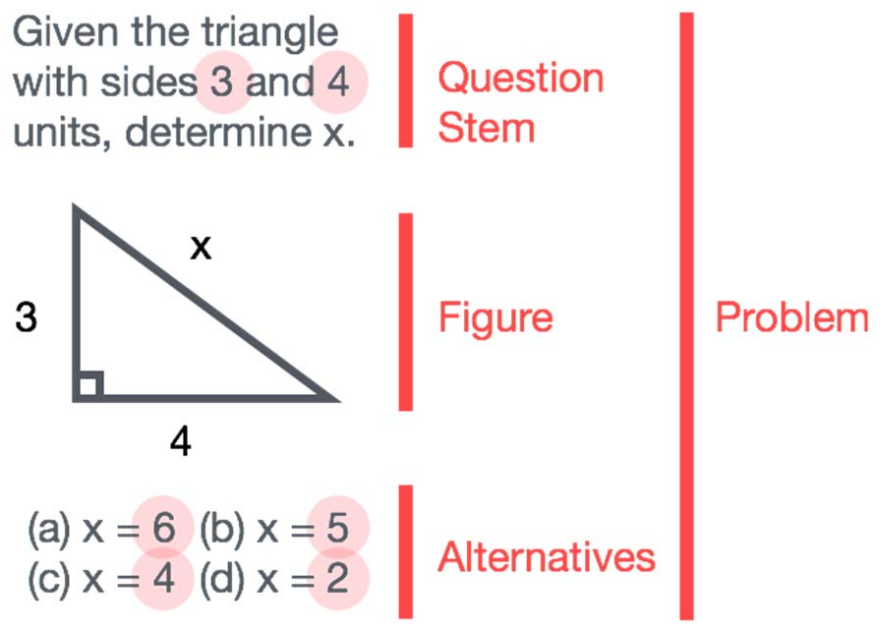
\includegraphics[width=0.25\textwidth]{images/quipid-problem.png}
            \caption{Quipid Problem Structure \cite{quipid}}
            \label{fig:quipid-problem}
        \end{wrapfigure}
        \indent A main goal for Quipid is to provide teachers with an easy way to assess students. Google Sheets is the backbone to achieving this goal. Quipid is designed with two sheets, a ``Problem'' sheet and a ``Formulation'' sheet. The Problem sheet is a library of questions and is linked to the formulation sheet. As Figure \ref{fig:quipid-problem} shows, a problem is made up of three parts: a ``question steam'', an optional ``figure'', and ``alternatives'', which are the multiple choice options for the question. The link between the formulation sheet and the problem sheet allows the formulation sheet to be programmed in such a way that when a teacher changes the parameters in the question stem, the alternatives are automatically updated.
        \smallskip
        
        Along with the formulation sheet, Quipid offers more programmability simply by virtue of using Google's G Suite (Google Sheets and Google Forms). Part of G Suite is a scripting language called Google Apps Script. This allows the user to program the Sheets and Forms with virtually infinite possibilities. Quipid leverages Apps Script to create the quiz in Google Forms based on the questions in Google Sheets, but a user of Quipid could program the tool to do any number of different tasks including integrating with third party tools, at which point the possibilities would be endless.  
        
    \subsection{Dysgu}
        The last work, Dysgu, is a concept more than an application. It was presented at FIE 2018 in a ``work in progress'' paper. It is presented as a collection of high level ideas without any concrete implementation. We mention it here because it is a platform in development with gamification features and some interesting ideas on student engagement.
        \smallskip
        
        Dysgu is described as an application for teachers to assign activities to students and track their progress. Students can sign in, interact with each other, and complete the assignments. There are three notable gamification features presented: scores and points, badges, and social awareness.
        \smallskip
        
        The paper describes the difference between scores and points as ``Scores are utilized to calculate student’s grade, whereas, points are used as currency in the system'' \cite{dysgu}. All students receive scores for completing activities, but they can earn points by achieving certain goals within the activities, such as being the first to complete an activity. The points earned can then be used in various ways throughout the system, like a time extension on an activity. 
        \smallskip
        
        Badges are similar to points. They are awarded for certain accomplishments and unlock features for the student like getting a sneak peek into an activity.   
        \smallskip
        
        The social aspect of the platform allows students to see how they are doing relative to the rest of the class. While everything is done anonymously, certain general statistics are made available to each student. For example each student can see the number of students to have completed an activity and each student will know which place they are in relative to their points. Also each student will be able to see the others' badges. 

\section{Design of Our System}
    Our platform is divided into a backend and a frontend. The backend handles the basic web app functionality along with all of the game logic and data storage. The frontend is responsible for dispaying data provided by the backend and processing user interaction. There is a very loose coupling between the backend and frontend. One advantage of having a loosely coupled back and front end is that they can be developed independently once an application programming interface (API) is agreed upon, allowing for quicker, parallel development. Another advantage is that either can be swapped out for a different technology should the need or desire arise as long as the new technology follows the same API.
    \smallskip
    
    An alternative approach would have been to write the frontend using the web framework's view implementation. The advantage with that approach is that the frontend would have greater visibility into and knowledge of the backend's data. This greater visibility comes at the cost of a potentially bloated system that could become difficult to change over time.
    \smallskip
    
    The overall platform design follows the microservice/model-view-template (MVT) pattern. Both patterns are well known and therefore will not be the focus of this paper (although we will briefly discuss certain architectural elements). Rather the design elements discussed here will be those specific to the actual game and not the surrounding architecture. In our implementation the backend is written in Python Django \cite{django} and the frontend is React \cite{react}.

	\subsection{Game Architecture}\label{architecture}
	    A game, at its core, is made of states, each representing a moment in the game with a specific functionality. We refer to this as Flow and Functionality. Flow is the progression from state to state and functionality is the operations that happen within each state. Our goal is to provide a flexible, programmable platform, so our focus throughout development has been to abstract out the flow and functionality of a game to provide as much control as possible to the user.

        \subsubsection{Flow}\label{flow}
	        Within a game our platform has seven states that can be arranged by the user in any order. The states are ``registration'', ``make\_teams'', ``standby'', ``questions'', ``leaderboard'', ``finished'', and ``hook''. Each state has logic in the backend that produces data to be displayed on the frontend. The flow of the game can be specified by the user and stored in the database as part of the game properties, discussed further in Section \ref{database}. Figure \ref{fig:architecutre-flow} shows an example of how states might be arranged in a particular game with two questions. In an alternate configuration, if the user wanted to use the same game but run through the questions quicker, they could remove the leaderboard state between the questions while everything else about the game remains the same, as seen in Figure \ref{fig:architecutre-flow2}.

            \begin{figure}[ht]
                \centering
                \begin{subfigure}[b]{0.45\textwidth}
                    \centering
                    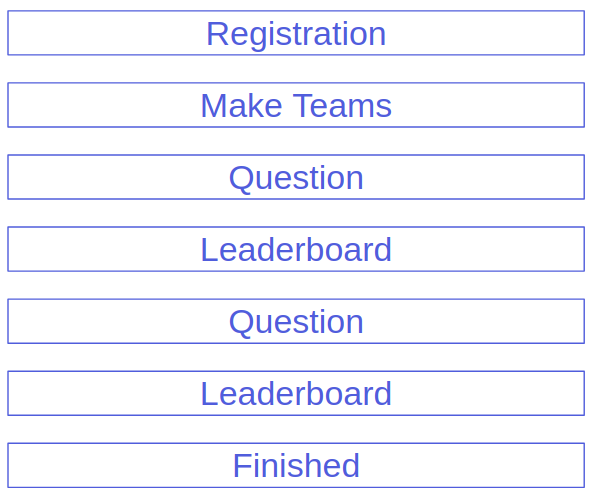
\includegraphics[width=0.8\textwidth]{images/architecture-flow.png}
                    \caption{Sample Game Flow Outline}
                    \label{fig:architecutre-flow}
                \end{subfigure}
                \begin{subfigure}[b]{0.45\textwidth}
                    \centering
                    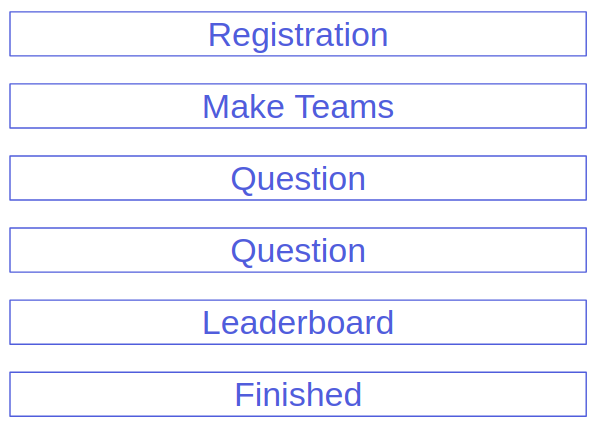
\includegraphics[width=0.8\textwidth]{images/architecture-flow2.png}
                    \caption{Sample Game Flow Outline Without Leaderboard State}
                    \label{fig:architecutre-flow2}
                \end{subfigure}
                \caption{Sample Game Flows}\label{fig:architecutre-game_flows}
            \end{figure}

            The ``hook'' state, called a flow hook, acts as a blank state where any behavior can be programmed to run when that state runs. Currently the flow hook backend state maps to the flow hook frontend state by specifying certain key values in the backend output in order to display it on the frontend. For example, specifying a value for the ``h1'' key in the payload from the backend will display that key's value in an h1 tag on the frontend. The current key options are h1, h3, h5, and p. We are hoping in the future to make the entire hook frontend page customizable as discussed in Section \ref{future-work}.
        
        \subsubsection{Functionality}\label{functionality}
            Functionality is the algorithms that run during each state. To give users access to the underlying functionality of a game, we have introduced the idea of hooks. A hook is a piece of user defined python code that will run when the user specifies it to run within the game flow. It is important to make a distinction between functionality hooks and flow hooks mentioned above. A flow hook is to be used when the user wants a custom view to be displayed during the game. A functionality hook is not a state itself, but rather runs in addition to the current
            \begin{wrapfigure}{r}{0.40\textwidth}
                \centering
                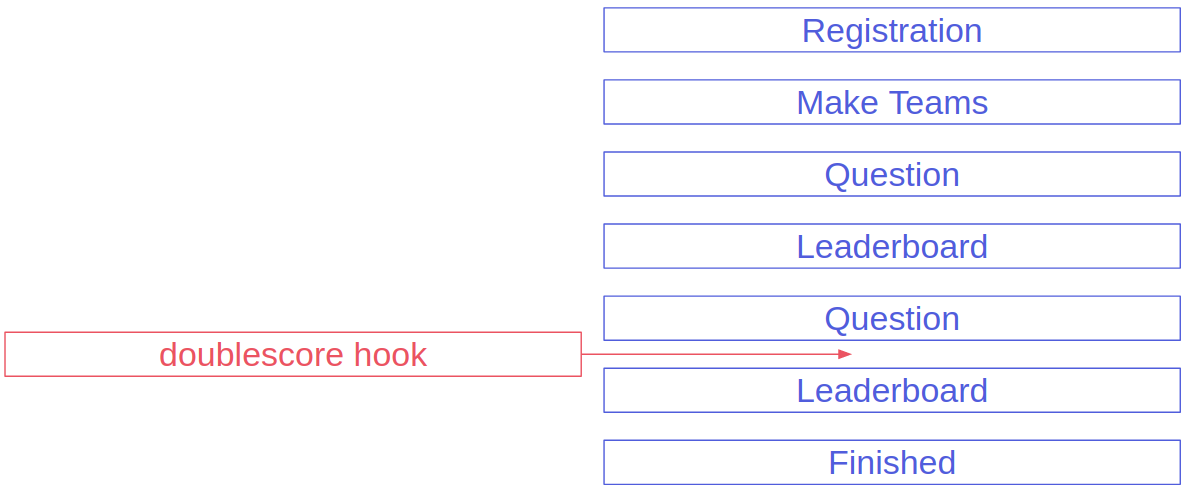
\includegraphics[width=0.40\textwidth]{images/architecture-hook.png}
                \caption{Adding a Functionality Hook to a Game Flow}
                \label{fig:functionality-hook}
            \end{wrapfigure}
            state.
            
            Figure \ref{fig:functionality-hook} shows how a functionality hook can be added to a game flow to run before the leaderboard state in order to double every player's points for the previous question. The user would need to define the algorithm for how they want to double all of the scores, but the example illustrates that this type of hook only alters the game's underlying data and does not require its own state with a frontend view like a flow hook. Functionality hooks can be run before or after any state. Each state should only need to run at most one hook before it and one hook after it, however it would be possible to insert empty flow hooks to run more hooks before or after a particular state.

	\subsection{Backend}
	    The server side code is written in Python using the Django web framework. We chose Django for our base framework for a number of reasons. First, Python is a familiar language that is good for rapid development because there is not a lot of boilerplate code required. Second, Python is a popular and well documented language and Django is a popular framework so any issues or gaps in our knowledge would likely have easily accessible solutions in either online forums or the Django documentation. Third, because of Django's popularity there are many external libraries that help extended its functionality. Two such libraries that we relied upon are Django REST framework (DRF) \cite{drf} and Django Channels \cite{channels}.
	    \smallskip

        During a game, communication between the client and server uses the websockets protocol. In the OSI model websockets is a layer 7 protocol and an alternative to HTTP. The reason for using this protocol is that it maintains a client/server connection, giving the server the ability to send data to the client without the client requesting it. This allows for two-way, real time communication between the client and the server and is a crucial part of a real time, interactive game like ours. Because websockets is a standard protocol, the implementations on both the front and back ends are straightforward. On the frontend no extra tooling is required - websockets support is build into React. On the backend, Django Channels abstracts out many of the finer details of websockets, providing an easy library to utilize the protocol.
        
        \subsubsection{The Game Object}\label{game-object}
            The brain of a game is the Game object. It is responsible for all game logic and communication. When first initialized it fetches all of the data from the database needed to run the game. This includes all of the questions, answers, game settings, and any custom code like functionality hooks. The game object extracts the game flow from the database and organizes the game accordingly. It runs through the states, from registering users to asking questions to scoring answers, and organizes the data that will be sent to the host and to the players for each state.
            \smallskip
            
            A major component of our platform is programmability through hooks. In addition to the hooks described in sections \ref{flow} and \ref{functionality}, we also provide scoring hooks so the user can customize how the game is scored for individual and team games. For hooks to be effective, they need to have access to the underlying data in the game object. Therefore, we pass references of the game object into every hook so that users are able to read and manipulate any of the game data. This provides users with limitless access to the backend, as if they were themselves developers.
            \smallskip
            
            The flexibility and customization that hooks provide comes at the cost of security. To open the system up to users also opens it up to bad actors. Currently we do not account for security concerns but it is worth noting that handling hook security is both critical and nontrivial. In order to make it more secure there is likely to be some amount of functionality loss, and although the extend is unknown, it seems unlikely to be significant. Nevertheless the security concern must be addressed.
	    
		\subsubsection{Libraries}
		    Part of our application's backend architecture relies on external libraries outside of the Django framework core. Three of these libraries play major roles in the design of the system and are worth explaining here.
            \\\\
		    \noindent{\emph{Django REST Framework}}
		    \smallskip

    	    Django REST framework extends Django to act as a RESTful API. This allows us to program RESTful endpoints on the server side so our frontend can call the server using standard web API calls to fetch and deliver information. Part of this process requires authenticating users and authorizing user access to data and resources. For this we elected to use JSON web tokens (JWTs).
            \\\\
    	    \noindent{\emph{Simple JWT}}
    	    \smallskip

    	    A DRF library that we use that simplifies the JWT implementation process called Simple JWT \cite{simplejwt}. There are five reasons why we chose JWTs. The first is that they are a modern and cutting edge authentication process, and when it comes to security it is important to be at the forefront of technology. The second is that it provides both authentication and authorization in one package, simplifying what can be a bulky and complicated process. The third is that they are fast, secure, and compact to generate and send between the client and server. The fourth is that a JWT is easily stored and renewed on the frontend and easily expired or revoked on the backend.
            \\\\
    	    \noindent{\emph{Django Channels}}
    	    \smallskip
	    
	        The backbone of the game functionality is Django Channels. It is the library we use as the websockets implementation on the server side. Channels simplifies communication between the server and clients, and allows us to specifically track, target, and distinguish communication between the game host and the game players. Figure \ref{fig:backend-libraries_channels} shows the basic Channels structure. The Game object (shown in blue) handles the game logic as described in Section \ref{game-object}.  When initializing a game, the host connects to the backend via websockets. Any information the host needs to display comes directly from that websocket connection.

            \begin{figure}[ht]
                \centering
                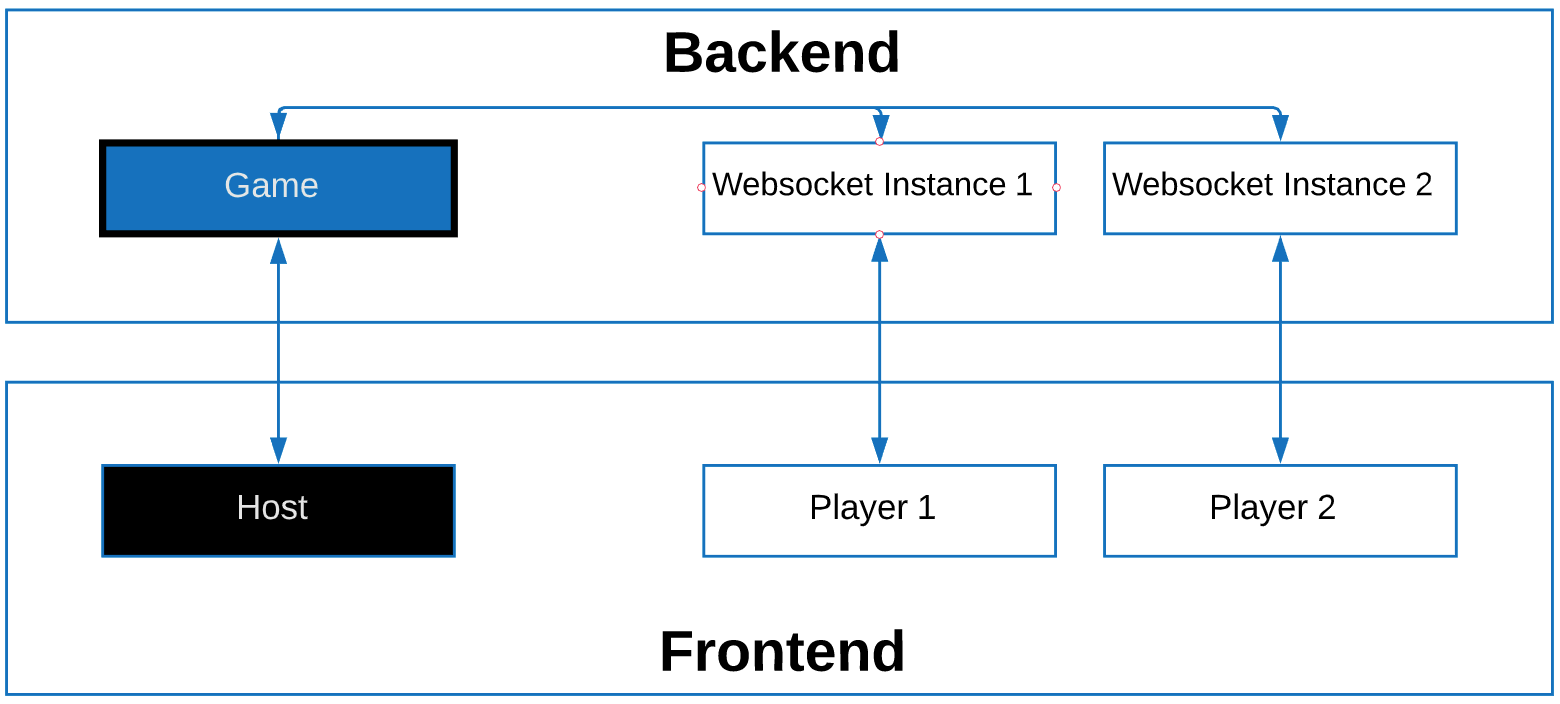
\includegraphics[width=0.8\textwidth]{images/backend-libraries_channels.png}
                \caption{Django Channels Game Structure}
                \label{fig:backend-libraries_channels}
            \end{figure}
            
	        Once the game is created, players can join through their own websocket connection. Each player has a separate connection to the server and their connection instance knows which game to communicate with based on the game pin they used to join. Upon first connecting to the game, each instance registers with the Game object, so the game has knowledge of and can reference each player instance individually, allowing it to send unique data to specific players. All data sent to the players starts in the Game object, then is sent to each player's websocket instance, and finally is forwarded to each player's frontend view. Similarly, data sent from each player to the game, for example when players answer a question, starts with user input on the frontend, is sent through the websocket connection to that player's websocket instance, and then forwarded to the Game object. There the information is processed accordingly and because each websocket instance is registered with the game, the game can properly attribute the data to a specific player.
	        \smallskip
	        
		\subsubsection{Database}\label{database}
    		Part of the backend's responsibilities is storing all of the system's data. This includes user names and passwords, games, game settings, questions, and answers. The database was designed with the goal of reusing as many objects as possible and follows third normal form as there are no funcitonal dependencies between table attributes. Figure \ref{fig:database-er_diagram} shows the Entity Relationship (ER) diagram of our database design.
    		
            \begin{figure}[ht]
                \centering
                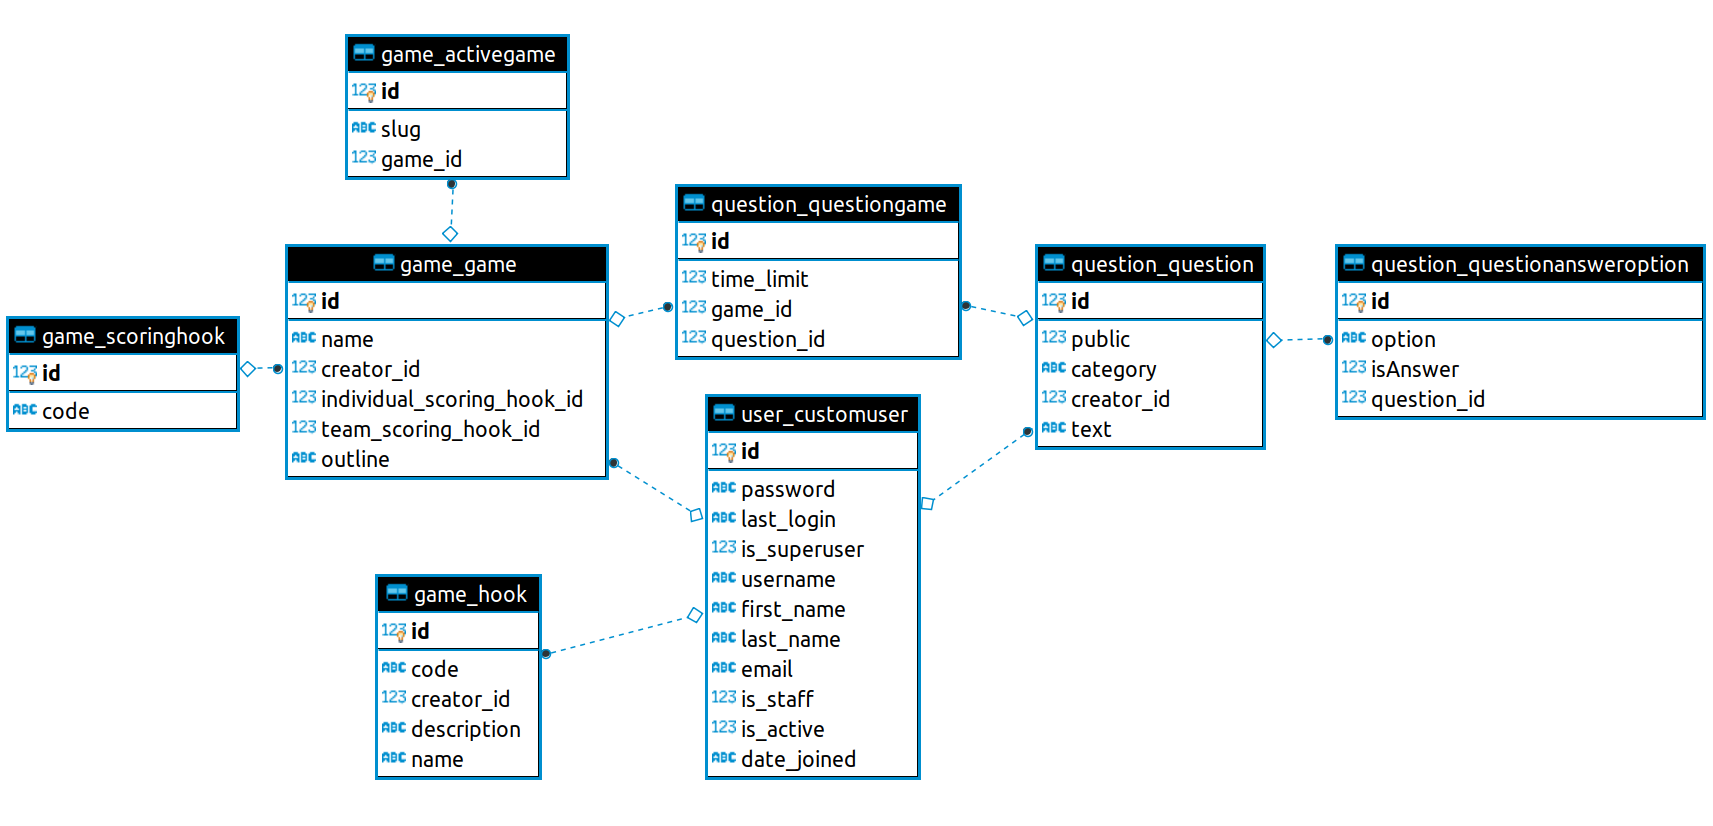
\includegraphics[width=0.9\textwidth]{images/database-er_diagram.png}
                \caption{Database Entity Relationship Diagram}
                \label{fig:database-er_diagram}
            \end{figure}
            
            It is helpful to think of the database as split into two sides, the question side, as in Figure \ref{fig:question-tables}, and the game side, as in Figure \ref{fig:game-tables}. The idea with this approach is that questions can be assigned to multiple games without the need to duplicate the question in the database.
            
            \begin{figure}[ht]
                \centering
                \begin{subfigure}[b]{0.45\textwidth}
                    \centering
                    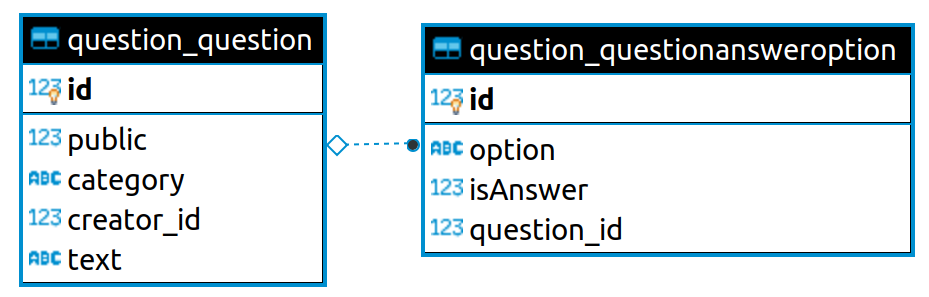
\includegraphics[width=\textwidth]{images/database-questions.png}
                    \caption{Question Tables}
                    \label{fig:question-tables}
                \end{subfigure}
                \begin{subfigure}[b]{0.45\textwidth}
                    \centering
                    \begin{separator}
                        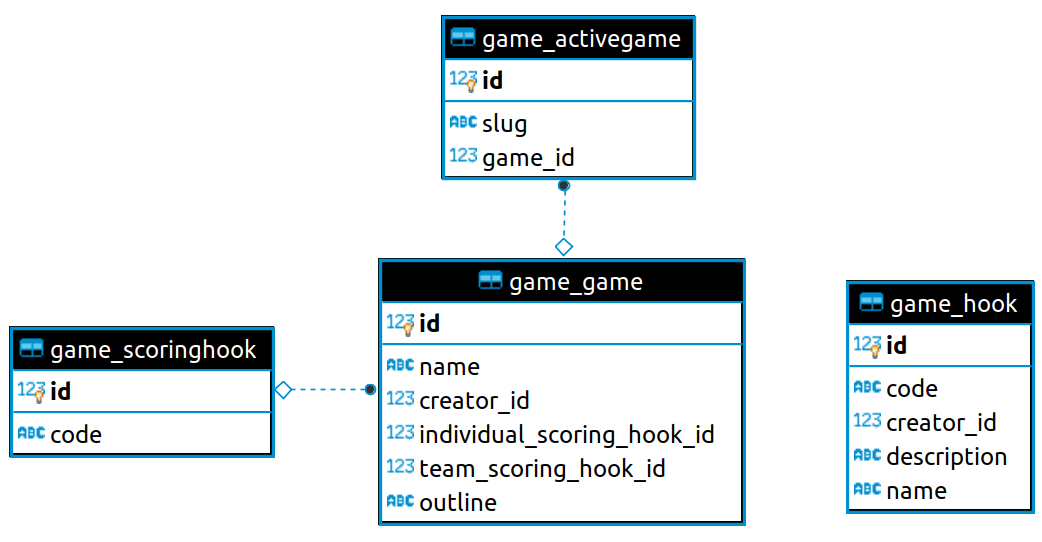
\includegraphics[width=\textwidth]{images/database-game.png}
                        \caption{Game Tables}
                        \label{fig:game-tables}
                    \end{separator}
                \end{subfigure}
                \\
                \begin{subfigure}[b]{0.9\textwidth}
                    \centering
                    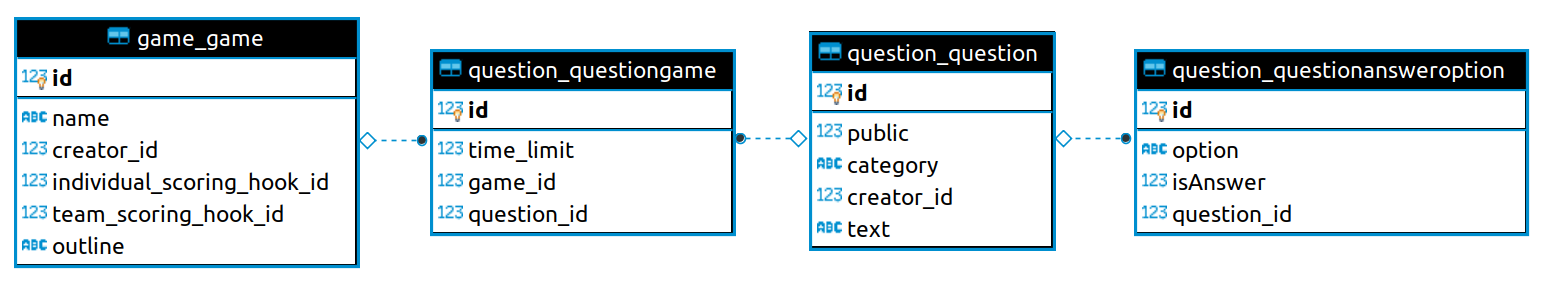
\includegraphics[width=\textwidth]{images/database-game_questions.png}
                    \caption{Question and Game Tables Relationship}
                    \label{fig:question-game-tables}
                \end{subfigure}
                \caption{Database Sections}\label{fig:database-sections}
            \end{figure}
    		
    		A question is made up of text, a category, and whether it can be publicly shared or private. A question's answer options are stored in a separate table with a foreign key (FK) relationship to the question. This design allows a question to have, in theory, an infinite amount of answer options. In the prior work referenced, answer options were typically limited to four or less, but our design removes that restriction. Answer options are assigned to a specific question and have a bit value indicating if they represent the answer to the question. This allows single questions to have multiple answer options.
    		\smallskip
    		
    		A flaw in this design is that the same answer option cannot be shared between questions because each option has a question id FK field.  To normalize this further we could add a junction table between the question and answer option so that the same answer options would not be duplicated in the database, however this approach seemed impractical because we did not want users having to search through existing answer options in order to add them to a question.
    		\smallskip
    		
    		The main game table contains game properties and customization features. The two scoring hook fields (individual and team) FK to the scoring hook table as shown in Figure \ref{fig:game-tables}. This allows for custom scoring algorithms to be written by our users and, if specified, will override the default scoring of our system as mentioned in Section \ref{game-object}. The reason scoring hooks are in a separate table is so that the user can reuse the same code in multiple games. For example, if a user writes an algorithm in a scoring hook to assign points based on the order the answers were submitted, they could write that once to the scoring hook table and then assign that same hook to multiple games.
    		\smallskip
    		
    		The outline column in the game table is where the game flow is stored. The functionality of the game flow is discussed in Section \ref{flow}. There are many ways the game flow could be stored in the database. One option would have been to create a separate table with an FK to the game table, an ordinal column indicating the order of the states, and a state column indicating the specific state. It would also need some way, either with more columns or another table, in order to reference functionality hooks. This approach was considered but ultimately declined because of the complexity. The approach chosen seemed reasonable and much more concise, although we loose data integrity validation in exchange for the simplicity.
    		\smallskip
    		
    		Our approach simply stores the game flow as a JSON string. While it is easier to corrupt this data, it provides much less overhead when storing and retrieving it and more importantly, allows for a more flexible shape of the data. Rather than relying on the database to ensure the data's integrity, we offload that responsibility to the front and back ends. When a game is fetched from the database, the game flow is retrieved from the outline column as a string and deserialized into its own data type.
    		\smallskip
    		
    		This approach works well because it does not require any joins when retrieving the data and it allows for the shape of the data to be fluid. For example, each state in the flow may or may not have a functional hook before it and after it. By storing the flow as a string, if these values are not present, we can ignore them completely by not including them in the JSON string. If this were stored relationally we would have needed nullable pre-hook and post-hook columns for each state, adding a lot of potentially wasted space.
    		\smallskip
    		
    		There are three tables in the database that are related to the game table which are the active game, the scoring hook, and the hook tables. Active games are games that are currently being played. They have an auto generated slug field that acts as the game pin so users can connect to it. The scoring hook table FKs to the game table and is used to store the code for both custom individual and team scoring.
    		\smallskip
    		
    		The last table related to the game table is the hook table. Interestingly, the hook table has no FKs to any other table (with the exception of the user table). This is because hooks do not belong to any one game and a game will have an unknown number of hooks. A junction table could be possible to connect hooks to games, but because of our outline design we elected for a different approach. In the hook table the creator and name fields must be unique together. That means that a single user cannot create two hooks with the same name. Because functional hooks are specified in the outline, it is there that the hook is referenced, namespaced using dot notation as ``creatorId.name''. For example if user 7 defined and wanted to use a functional hook called ``doublescore'' they would include it in the outline JSON as ``7.doublescore''. This way when the outline is deserialized, the hooks are parsed and the hook table is queried by creator id and name in order to fetch the hook's code.
    		
    		The question and game tables are joined using the question-game junction table, illustrated in Figure \ref{fig:question-game-tables}. This table represents questions being assigned to games. It has time limit field as well so that question times are only specific to games and not questions. This allows the same question object to be used more flexibly. If a question's time limit was specified in the question table, then a duplicate tuple would need to be created just to change the time.

	\subsection{Frontend}
	    The frontend is written in React with Redux \cite{redux}. There is little logic in the frontend related to gameplay because the game is controlled on the server side. The frontend's main purpose is to present information from the server to the users and send input from the users to the server. We chose React as our frontend architecture because it is a modern frontend framework and therefor designed to consume APIs. It also helps keep our frontend code organized and React components allow us to reuse code, ultimately leading to a cleaner code base and more rapid development. Starting this project we also understood that React had a reputation for fast rendering which is an appealing feature when creating an online game like ours.
	    \smallskip
	    
	    At this stage in development Redux is not widely used throughout our system. We use it on the ``non game/non websockets'' side of the frontend to make information globally available to components. One such use case is with the user's JWT. It is useful to have this value available globally because it is needed for every HTTP API call. When playing the game itself, however, we do not use Redux at all. The reason for this is that during a game information typically comes from the backend when it is needed and discarded when the game state changes, so there is no need to use a global store for information. That is not to say that it is not possible to use Redux within the game, but a decision to do so would be more stylistic than functional.
	    
	    \subsubsection{User Experience} \label{ux}
	        There are two different types of users for our system, a host (sometimes referred to as a teacher) and a client (sometimes called a player or a student). The role of the user will determine the user experience. Upon first entering the site, users are given the option to login or join a game, as shown in Figure \ref{fig:frontend-login}. If a user has an account they are assumed to be a teacher and can host a game. If they want to join a game they assume the player role. We have future plans to allow non-teachers to login as well, which will be discussed in greater detail in Section \ref{future-work}.
	        
            \begin{figure}[ht]
                \centering
                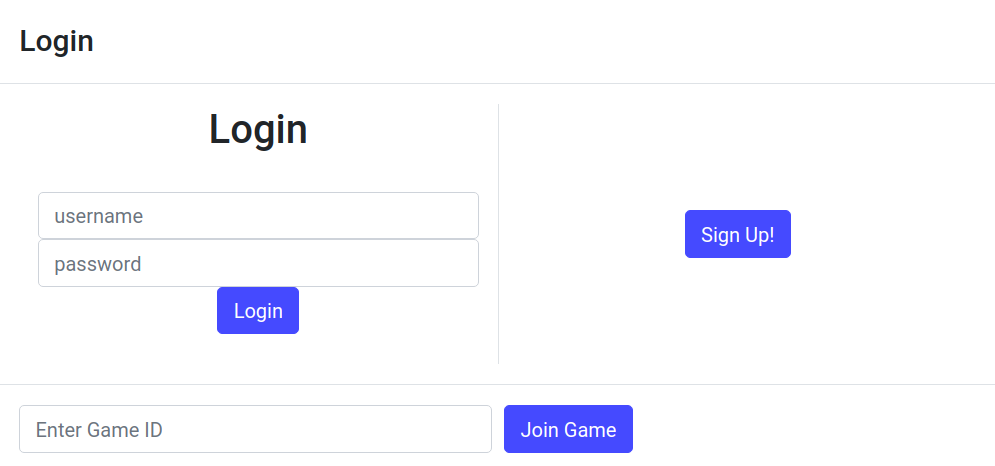
\includegraphics[width=0.8\textwidth]{images/frontend-login.png}
                \caption{Login Modal}
                \label{fig:frontend-login}
            \end{figure}
            
            Once a host logs in they are presented with their home dashboard. In our current state not all dashboard functionality is implemented, however in theory the host would be able to create, read, update, and delete (CRUD) all of their games, questions, and hooks. In addition they could search for, copy, and play public games.
            \smallskip
            
            In order to play a game they would navigate from their home dashboard to their game dashboard. Shown in Figure \ref{fig:frontend-games_dashboard}, the host is able to select which game they want to play and which mode to play it in, team or individual. Team mode defaults to two teams, but with the dropdown menu they can select up to 20. Once the game is selected, a websocket connection is established between the host and the server and the game object is instantiated with all of the game's information.  
            
            \begin{figure}[H]
                \centering
                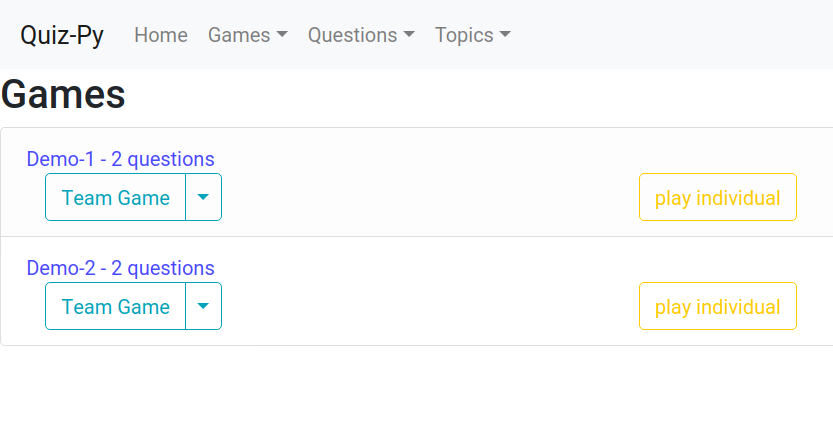
\includegraphics[width=0.5\textwidth]{images/frontend-games_dashboard.png}
                \caption{Host Game Dashboard}
                \label{fig:frontend-games_dashboard}
            \end{figure}
            
            The flow of the game once it is instantiated depends entirely on how the host programmed the game. The following explanation describes the default behavior for states and their outputs, however this behavior is easily overridden at which point the game could progress completely differently.
            \smallskip
            
            The game would then likely move to the registration state where players are presented with the game pin and able to join, as seen in Figure \ref{fig:frontend-join_game}. After entering their names, players enter the standby state. Once the host is ready, they click the ``ready'' button and the game progresses to the next state. This would typically be either make teams if it is a team game, or the question state if it is an individual game, although this is not required. When in the make teams state, after the teams are organized by the server, the host will display all of the teams and their rosters while the players will each receive the name of their team on their devices. 

            \begin{figure}[H]
                \centering
                \begin{subfigure}[b]{0.49\textwidth}
                    \centering
                    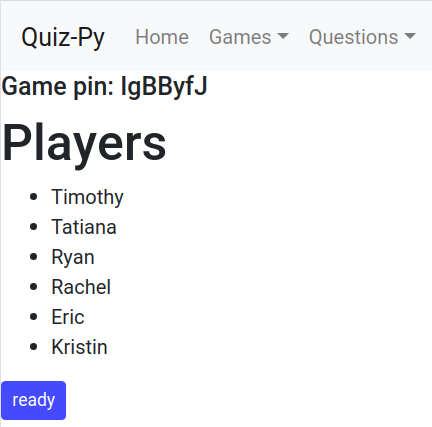
\includegraphics[width=0.5\textwidth]{images/frontend-join_game.png}
                    \caption{Join Game}
                    \label{fig:frontend-join_game}
                \end{subfigure}
                \begin{subfigure}[b]{0.49\textwidth}
                    \centering
                    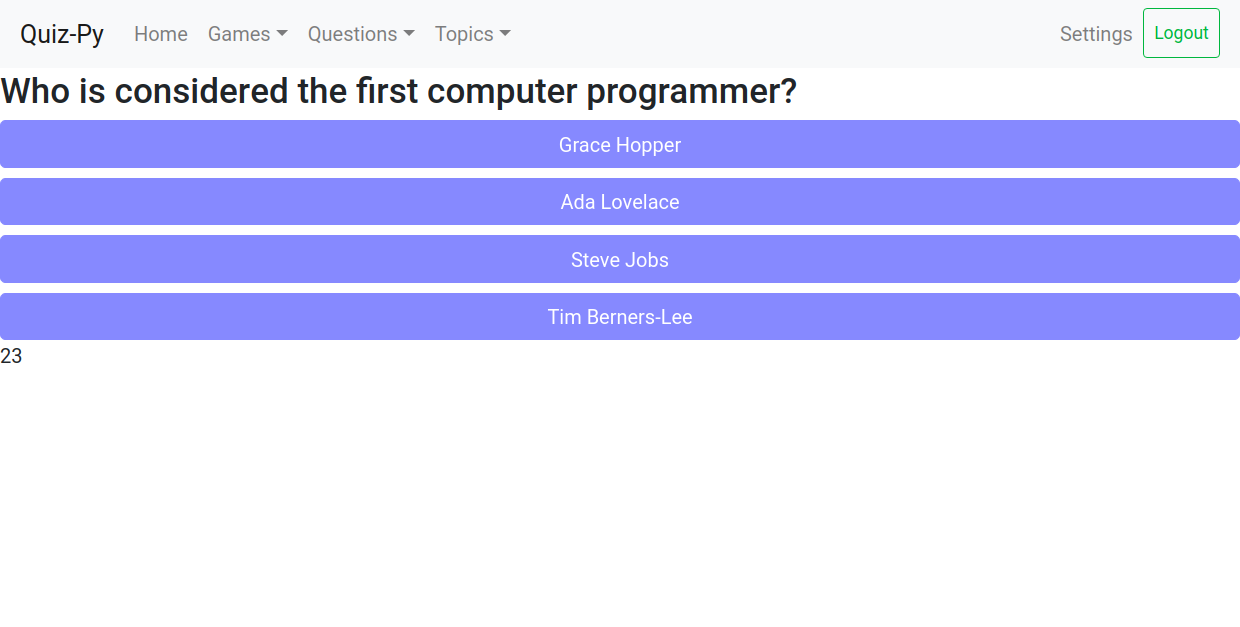
\includegraphics[width=0.9\textwidth]{images/frontend-question.png}
                    \caption{Game Question}
                    \label{fig:frontend-question}
                \end{subfigure}
                \begin{subfigure}[b]{0.49\textwidth}
                    \centering
                    \vspace{3mm}
                    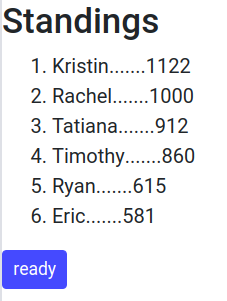
\includegraphics[width=0.35\textwidth]{images/frontend-standings.png}
                    \caption{Game Standings}
                    \label{fig:frontend-standings}
                \end{subfigure}
                \begin{subfigure}[b]{0.49\textwidth}
                    \centering
                    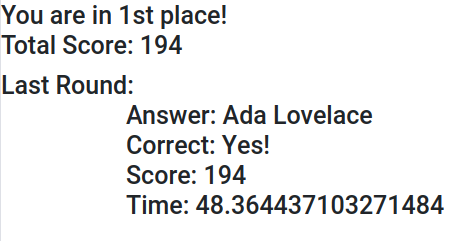
\includegraphics[width=0.9\textwidth]{images/frontend-player_summary.png}
                    \caption{Post Question Player Summary}
                    \label{fig:frontend-player_summary}
                \end{subfigure}
                \caption{In Game Views}\label{fig:frontend-user_interface}
            \end{figure}
            
            
	        In the question state the view is the same for the host and students, as shown in Figure \ref{fig:frontend-question}, except students do not see the timer on their screen. Once all of the students answer or time runs out, the game progresses to the next state. If that is the leaderboard state, then the standings page displays the player rankings on the host screen, seen in Figure \ref{fig:frontend-standings}. At the same time each player can see their own personal summary on their device, shown in Figure \ref{fig:frontend-player_summary}. When the finished state runs, the view for the host and players is similar to that of the leaderboard state.
	    
	    \subsubsection{Game Architecture}
            The game architecture is split into two sections, the host and the client. The two sides are similar because they both need to process and display the same state data, however there are minor differences, like for example when the host needs to display a timer. The host and clients also receive differently shaped data for any given state, so it is necessary to split them, mirroring the backend architecture.
            \smallskip
            
            Data coming in on both sides goes through the same filtering process in order to render the correct page. The payload includes a state field that is read and matched on, forwarding the data to and rendering the corresponding frontend page, as illustrated by Figure \ref{fig:frontend-pages}. The frontend always responds to the state is is sent and never sets its own state. This structure allows the server to be in full control of the game, always aware of which state the game is in and always able to change the state at any time.

            \begin{figure}[ht]
                \centering
                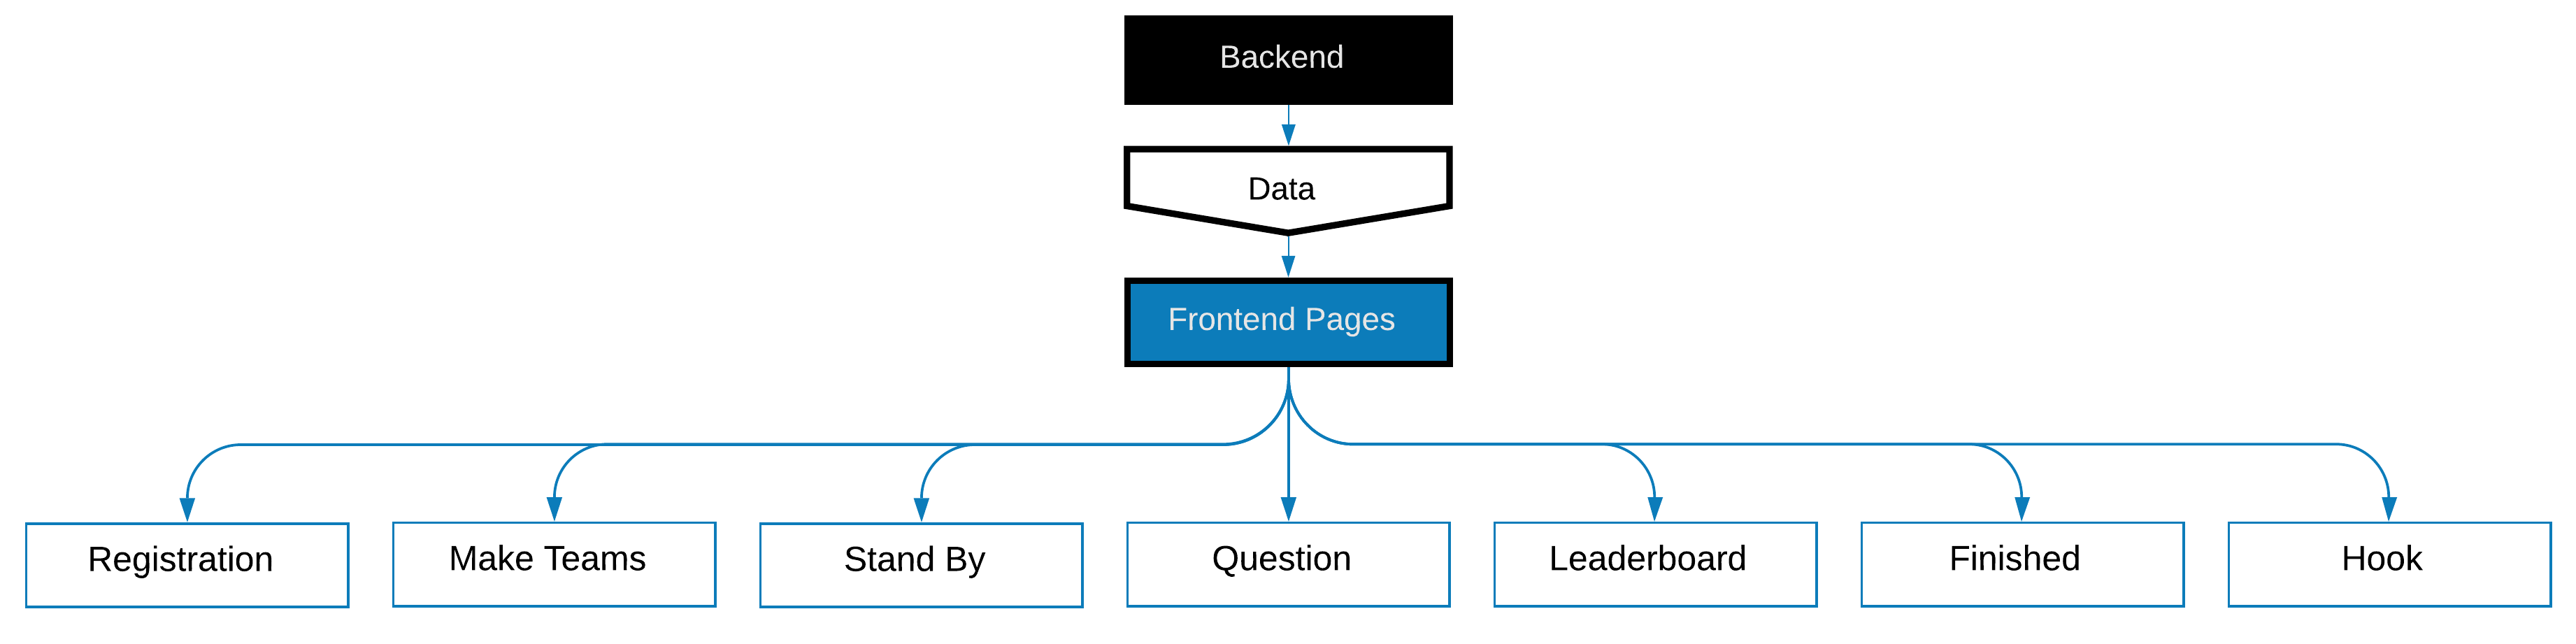
\includegraphics[width=0.9\textwidth]{images/frontend-pages.png}
                \caption{Filtering Data to Pages}
                \label{fig:frontend-pages}
            \end{figure}
            
            It is important to distinguish between the server controlling the state and the frontend sending events to the server, like time running out during a question or the host clicking a button to start the game. These events are registered on the frontend and sent to the server, but it is the server, not the frontend, that decides how to process these events and what the next state of the game will be.
            
            \smallskip
            There are three ways for the frontend to indicate the completion of a state to the server. The host can hit the ``next'' (or ``ready'' depending on the page) button, all of the students could have submitted an answer during a question, or the timer can run out during a question (or any other state as it is possible to add a timer to any host page through the use of hooks).

\section{Development}
    Development for this platform took place over a 14 week period. When starting we did not have a plan to follow any traditional development processes, nor did we adopt one as the project grew, however as we progressed our own process organically emerged that could loosely be defined as Agile.
    \smallskip
    
    Traditional development processes can be difficult to implement by one or two people just starting a project. For example, Waterfall requires designs up front and releases when a feature is complete but for a new project its design and direction may be unclear and there might be nothing to release once a feature is complete. Agile also contains some structure that is difficult for a new project, such as daily stand-ups and a scrum board to track features and progress. A new project might start as a hobby and programming might happen sporadically when it is convenient. Or new features might be added only when they are thought of and a scrum board would not serve any purpose. For these reasons we did not adhere to any particular process but instead we let our own process emerge.
    \smallskip
    
    For our project we met once a week to give status updates. We started this schedule out of necessity, following the class schedule, but as time went on we found the meetings helpful for the development process and continued with them even when school was out of session. Typically I would start by presenting the progress that I made since our last meeting and Dr. Hajja would offer positive and negative feedback. If I had any technical difficulties during the previous week, I would bring them up and we would try to work through them together. Then we would have a brainstorming session where we would think of new features that should be added to the platform. While we could both contribute, most of the vision and feature ideas for this project came from Dr. Hajja. Lastly we would make a general plan about what was to be accomplished for the next week. This plan was never set in stone and we were always willing to adjust, but nonetheless, we usually hit our weekly goals.
    \smallskip
    
    In some sense this process could be considered Agile. Our sprints lasted one week and Dr. Hajja's role could be compared to an Agile Product Owner because he would give feedback about how features were implemented and what features were to be added next. My role would certainly be considered the developer as I mostly implemented features. We did not have any way of tracking or pointing features as one would expect in Agile, but I did keep an informal list of features in a text document that I would occasionally reference when looking for the next feature to add.
    
\section{Future Work}\label{future-work}
    As the US Defense Innovation Board says, ''software is never done" \cite{mcquade}. The only reason we stopped development when we did was because of time and scheduling constraints, however there is a virtually endless list of features that can be added to the system. Here we highlight some of the more interesting and pressing features that we hope to add in the future.
    \\\\
    \noindent{\emph{User Interface}}
    \smallskip
    
    Our focus up to this point has been on game functionality. The user interface (UI) that currently exists was stood up quickly just so we could test new features. It will be necessary to develop the UI further so we maximize the overall user experience.
    \\\\
    \noindent{\emph{Deployment}}
    \smallskip

    All of the work for this project has been done locally. There have been no attempts up to this point to deploy the application. Of course, we will need to deploy it at some point if we want a usable product. We will likely use Heroku as our hosting platform because it requires relatively little setup and they offer free accounts.
    \smallskip
    
    There are a few concerns for when we deploy. The first is that using websockets could complicate our Heroku configuration. We will have environment variables such as websocket URLs that will likely need to be automatically set and loaded from a configuration file. Also, in addition to our standard database, Django Channels uses Redis so we will need to figure out how to deploy and connect to Redis using Heroku. 
    \\\\
    \noindent{\emph{Finish API}}
    \smallskip
    
    Since building out the API our design has changed but the API did not get updated. In order to finish the UI it will be important to first finish the API. This means making all appropriate endpoints so users can CRUD their data. 
    \\\\
    \noindent{\emph{Premade Hooks}}
    \smallskip
    
    With the amount of programmability in our system we run the risk of alienating non-technical users. Ideally we would like our platform to be used by technical and non-technical users alike, allowing them as much control and programmability as they want. At this point we offer customization but we do not have any resources for users that just want it to work without any programming. Therefor we would like to include pre-made code that packages certain functionality, such as different scoring hooks, that can be easily dropped into any game so the non-technical user does not have to worry about programming but could still change default functionality.
    \\\\
    \noindent{\emph{State Hook Frontend}}
    \smallskip
    
    As mentioned in Section \ref{flow}, we offer a programmable flow hook but the frontend can only display certain text/fields. We would like to open up the frontend to be completely programmable as well, however more research needs to be done as to how to actually implement this. Some questions that needs answers are: our frontend is in React, so would to user write custom react, or would we limit it to HTML? If HTML, could we use javascript inside of it? With either implementation, how would variables coming from the backend be handled? What kind of security would we need to put in place to avoid bad actors or good actors that made a mistake? Currently we do not have a proof of concept for this work, so we have many questions as to the feasibility of this idea as well as how it would be implemented.
    \\\\
    \noindent{\emph{Question Types and Media}}
    \smallskip
    
    We saw in Section \ref{kahoot} that the Kahoot platform offers a variety of different question types along with an option to add images and videos to the question. We like this feature and would also like to extend our platform to offer similar options. Because we want to give users as much control as possible, an idea would be to allow the user to program their own question type, however this idea is in its infancy and further testing would need to happen in order to determine its viability.
    \\\\
    \noindent{\emph{Change Answer}}
    \smallskip
    
    When a student answers a question their state automatically changes to the standby state. This means that it is not possible for a player to change their answer, even if the host tried to program this functionality in a hook. It would be nice to give the host the option to allow students to change their answer while there is still time left on the question. And ideally the host would be able to set a limit to how many times a student could change their answer or make it unlimited. Implementing this feature would not be a small amount of work because we would need to revisit the process for what happens when a student answers a question and potentially make big changes to this process. There is also a chance that we would have to introduce another state. Lastly, there is currently no customizable way for the host and players' states to be different. As mentioned, when a player answers their state moves to standby while the host remains in question, but this happens automatically. This feature would possibly require the host to be able to specify the host state and the player state at any given time, a customization that currently does not exits.
    \\\\
    \noindent{\emph{Move Backwards}}
    \smallskip
    
    Another feature related to states is the ability for the host to move backward in the game. There are questions that arise from this idea, such as if they move back to a question, do the redo the question or just see it? But in anticipation for this feature we already keep a list of previous states in the game object, so while that is by no means a major step towards implementing this feature, it does provide some scaffolding for future work.
    \\\\
    \noindent{\emph{Player Accounts}}
    \smallskip
    
    As discussed in Section \ref{ux} we would like players to be able to join a game under their own account rather than anonymously. This could provide an explosion of more features related to teachers grouping students into classes and tracking their progress. In order to implement this feature we would need to include an optional user id in the game object alongside the player's name, this way the game would know who is playing the game and be able to report their performance accordingly.
    
\section{Conclusion}
    We have explained how our platform works and looked at existing platforms and the features they offer. While there are similarities between ours and those that exist, there is not one that offers as much flexibility and customization as ours. Our novel idea of giving users access to the underlying game data through the use of hooks sets our platform apart and allows users more options than any other product we have seen. By offering this flexibility we hope that teachers will be able to further engage their students in creative ways that we have not considered. 

\printbibliography[title={Bibliography}]


\end{document}

